\chapter{Implementation as an Agent-Based Model} \label{chapter-agent-implementation}

In this chapter we document the implementation of the core agent-based model using the `Overview, Design concepts, and Details' (ODD) standard \cite{grimmODDProtocolReview2010a} The objective of the standard is to assist researchers in making model descriptions sufficiently complete and explicit that the model can be reproduced. The standard was originally envisioned as a protocol for describing ABMs in ecology, but it has been widely used in other fields.

Although we have explained a great deal of the theory behind the model and even specific modelling decisions in the previous eight chapters, applying the ODD protocol allows us to make explicit the computational structure of our model and rthe way the agnets are implemented. Following Grimm et al. \cite{grimmODDProtocolDescribing2020} this ODD consists of seven elements: % {(Figure 1)}:allows us

\begin{enumerate}
    \item Purpose
    \item State variables and scales
    \item Process overview and scheduling 
    \item Design concepts
    \item Initialization
    \item Input and 
    \item Submodels 
\end{enumerate}
% Conceptually the elements fall into the three categories ``Overview,'' (1-3) ``Design concepts'' (4, with subcategoriessoecific modelling d)  and ``Details''; hence the acronym ODD.
% The exposition in this chapter is strictly descriptive and what the model includes and does.


%Chapter~\ref{chapter-methodology}, on methodology, gives more detail on the modelling purpose, strategy, and type. The formulae used in the model are described and explained in Chapter~\ref{chapter-model}, the model chapter. Appendix~\ref{appendix-parameters} provides parameter values.  


\section{Purpose}
% TODO add in purposes of modelling work - The purpose of this model is to understand ..Following xyz, xyz gives x purposes for modellingr
The purpose of this ABM is to provide a representation of city development subject to financialization, where financialization refers to the purchase of land and housing by owners of capital. More specifically, we seek to understand the links between financialization and the distribution of housing ownership, the capture of rents, and urban productivity. 

The model  is intended to combine a theoretically correct simulation of the spatial and temporal growth of a city with a new model of a housing market in which individual agents buy and sell property, live, work, and retire subject to a realistic financial system. 
%, through financialization of the urban housing market. 


%Our goal is to examine how financial decisions affect home ownership while black-boxing the transmission of agglomeration effects through firms from aggregate productivity gains to population growth.

\section{State variables and scales}

\begin{figure}[h!tb]
    \centering
        \resizebox{\textwidth}{!}{
\tikzset{AgentStyle/.style={red, draw=black, font = {\Large\bfseries\sffamily}}}% Style for main lablels
\tikzset{TStyle/.style={red, font = {\Large\bfseries\sffamily}}}
\tikzset{ImmigrantStyle/.style={ purple!50!blue!70,  font = {\Large\bfseries\sffamily}}}
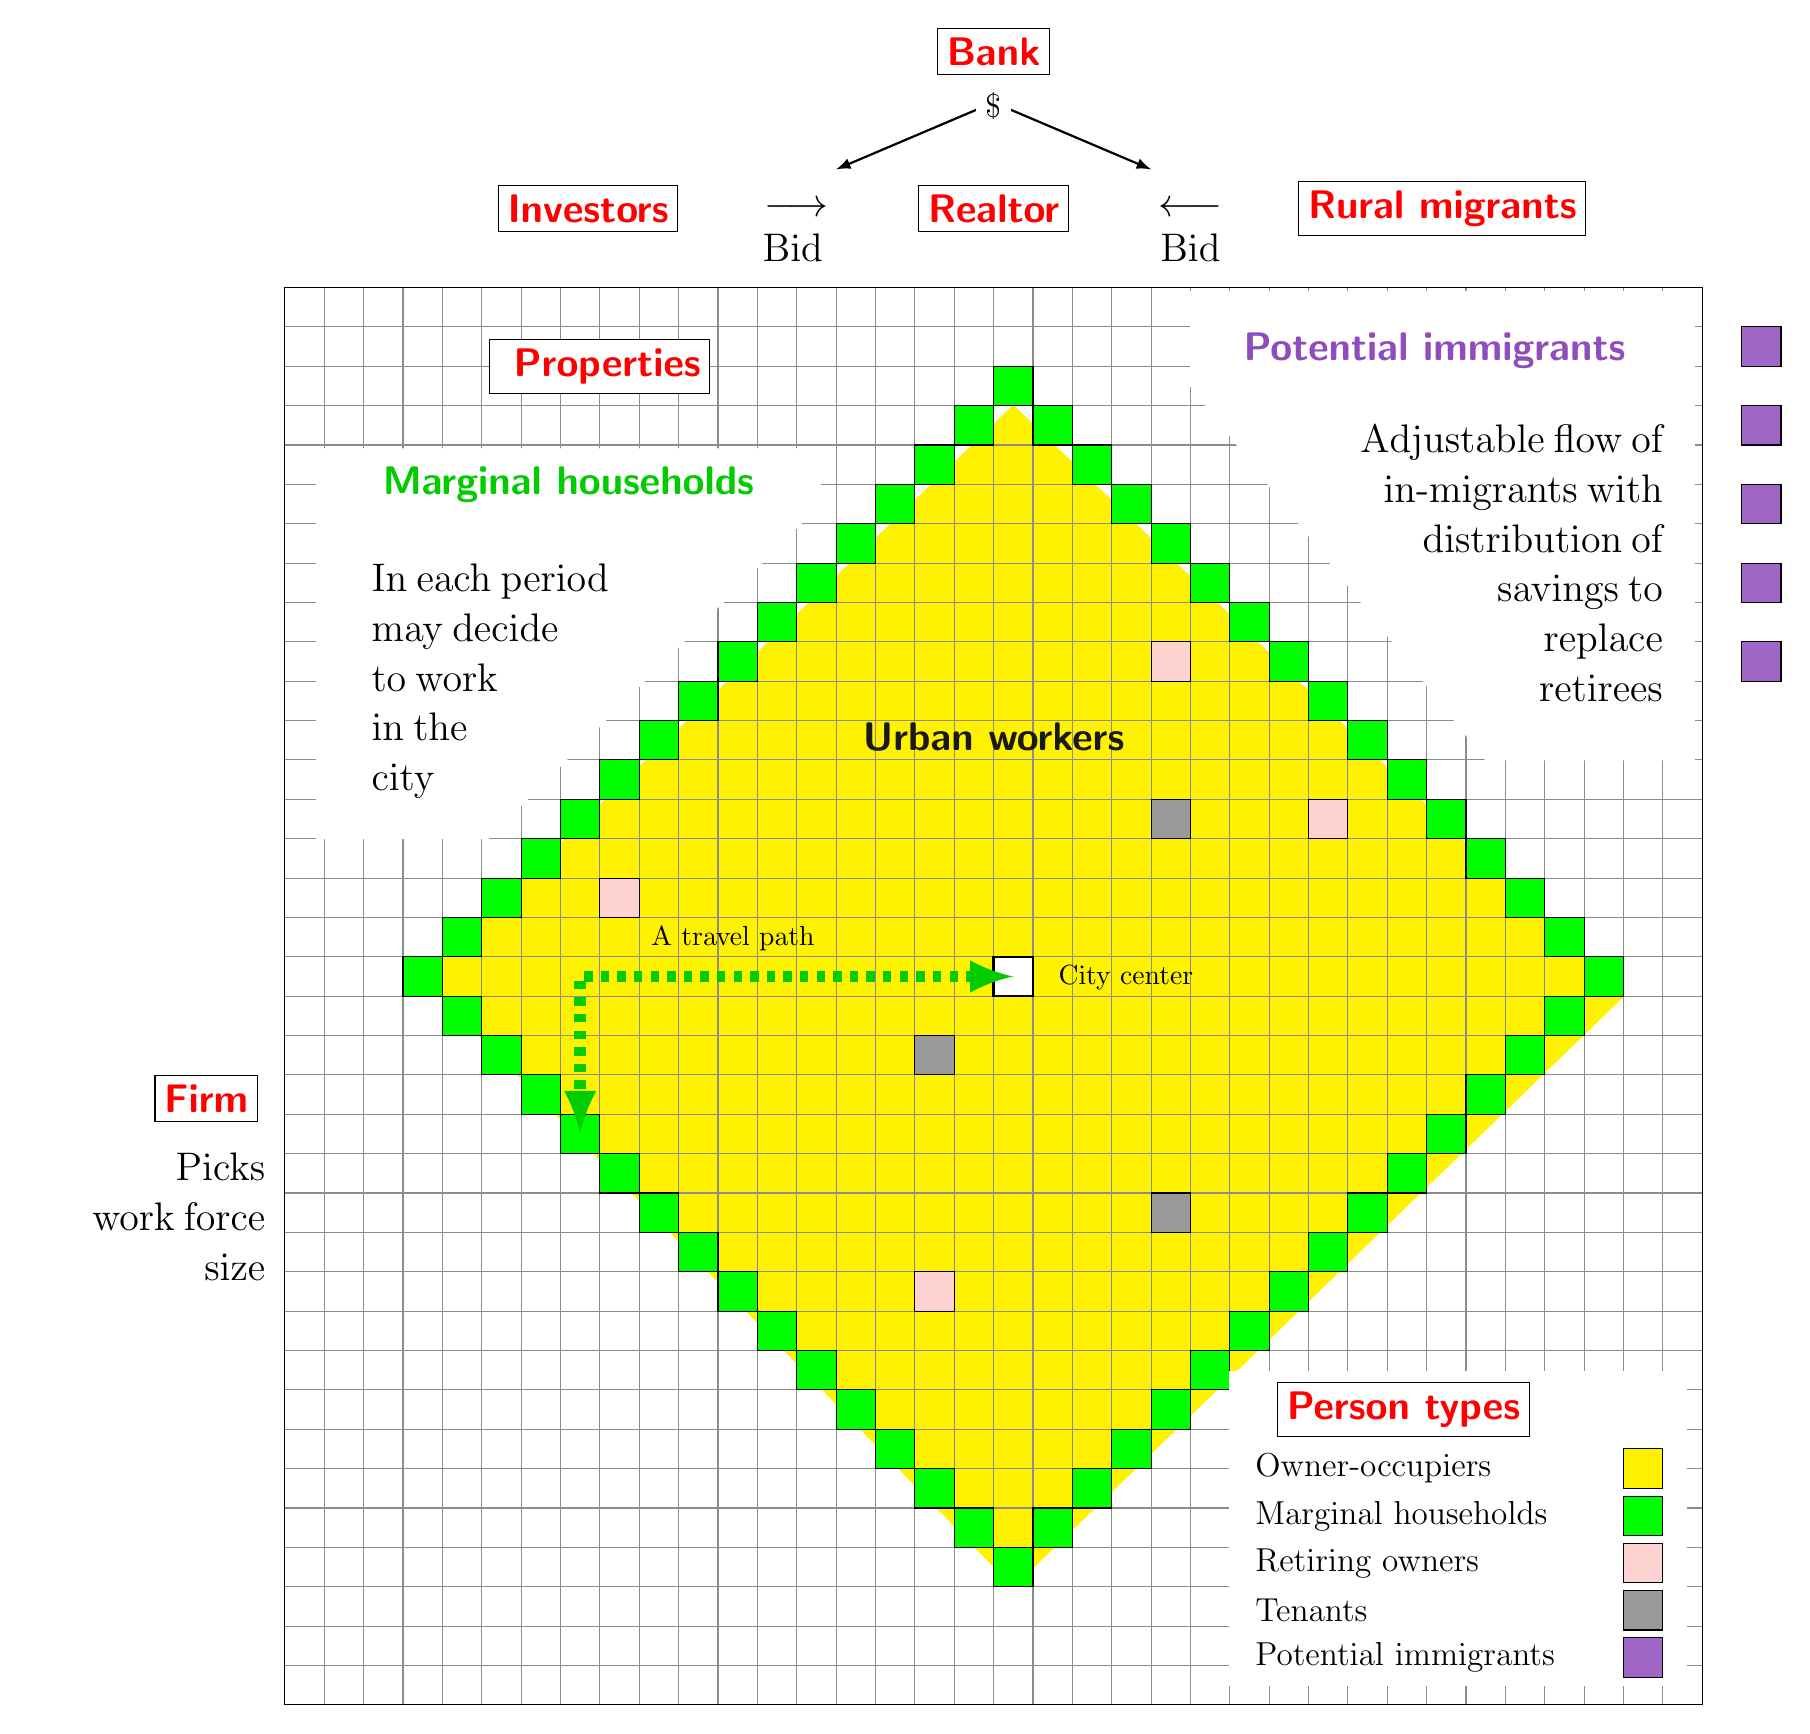
\begin{tikzpicture}
%\draw[very thin, gray!50, step=.5](-10,-10)grid(10,10);
% Locations for main label
  %Yellow square
 \draw [fill=yellow!80, yellow](8,0)--(.25,7.5)--(-7.25,.25)--(.25,-7.5)--cycle;  
 
 % grid 
  \draw[ thin, gray!90, step=.5](-9, -9)grid( 9, 9);
  \draw[  black, step=.5](-9, -9)rectangle( 9, 9);
  % center
 \draw  [fill=white, thick]  (0,0) rectangle +(.5,.5);
  \node at (1.68, .23) { City center};
  
% Marginal  residents _the green boundary
\foreach \z in {-7.5,-7,...,0}{ \draw  [fill=green] (\z,  {7.5+\z} ) rectangle +(.5,.5);} 
\foreach \z in {0,.5,...,7.5}{ \draw  [fill=green] (\z,  {-7.5+\z} ) rectangle +(.5,.5);}
\foreach \z in {-7.,-6.5,...,0}{ \draw  [fill=green] (\z,  {-\z-7.} ) rectangle +(.5, -.5);}  
\foreach \z in {.5,1,...,7}{ \draw  [fill=green] (\z,  {7.5-\z} ) rectangle +(.5,.5);}

% travel path
\draw [line width=1.5mm, latex-latex, dashed, black!20!green](.25, 0.25)--(-5.25,0.25)--(-5.25,-1.75);
\node at (-3.31,.73) {A travel path};


%.  Marginal households
\begin{scope}[shift={(-.4,0)}]
    \draw [fill=white, white] (-8.2, 6.95) --(-1.8,6.95)--(-1.8,6.25)-- (-6.02, 2)--(-8.2,2)--cycle;
    \node at (-5,6.5)[TStyle, black!20!green!100]{Marginal households}; 
    \node at (-5.5,4.)[text width=4cm] {\Large In each period \\may decide \\to work\\ in the\\ city\par};
\end{scope}
 
%  Firm
\begin{scope}
    \node [AgentStyle] at  (-10, -1.3){Firm};
    \node [text width=2.9cm, fill=white, align=right] at (-10.7, -2.8) {\Large Picks\\ work~force\\ size\par % \\normalsize(partial adjustment)
    };
 \end{scope}
 
 %Immigrants
     \begin{scope}[shift={(0,0)}]
     \draw [fill=white, white] ( 2.5,8.95) --(8.9, 8.95)--(8.9,3)-- (6.25, 3)--(2.5, 7.75)--cycle;
    \node at (5.6,8.2)[ImmigrantStyle]{Potential immigrants}; 
     \node [text width=6cm,  align=right] at (5.5,5.5) {\Large Adjustable flow  of \\ in-migrants with distribution of\\savings to\\ replace\\ retirees\par };
\end{scope}

% Locations for resident agents. (The first of these numbers is for the key.)
\def\retirees   {(2,4), (-5.,1), (-1,-4), (4,2)};			% retirees,   
\def\migrants {(9.5, 8), (9.5, 7),  (9.5,6.), (9.5,5.),   (9.5,4.)}; 	%potential migrants
\def\rental      { (2,2), (-1.,-1), (2.,-3)}; 			%rental properties

% Drawing resident agents.
\foreach \p in \retirees  {\draw [fill=pink!70] \p rectangle +(.5,.5);};
\foreach \p in \rental     {\draw [fill=black!40] \p rectangle +(.5,.5);};
\foreach \p in \migrants    {\draw [fill= purple!50!blue!60] \p rectangle +(.5,.5);};

% Labels and drawing for key for resident agents.
\begin{scope}[shift={(-.5,0.25)}]
    \draw [fill=white, white] ( 3.5,-5.02) rectangle (9.3,-9);
    \node at (4.1,-5.5) [right, AgentStyle]{ Person types};  %Title for key
    \node at 		(3.7,-6.25) [right]		{\large Owner-occupiers};
    	\draw [fill=yellow]    (8.5,-6.5) rectangle +(.5,.5);
	
    \node at 		(3.7,-6.85) [right]		{\large Marginal households};
    	\draw [fill=green]     (8.5,-7.1) rectangle +(.5,.5);	
	
    \node at 		(3.7,-7.45) [right]		{\large Retiring owners};
    	 \draw [fill=pink!70] (8.5,-7.7) rectangle +(.5,.5);
      
    \node at 		(3.7,-8.05) [right]		{\large Tenants};
    	\draw [fill=black!40  ]  (8.5,-8.3 ) rectangle +(.5,.5);	
	
    \node at 		(3.7,-8.65) [right]		{\large Potential immigrants };
    	\draw [fill= purple!50!blue!60]  	    (8.5,-8.9 ) rectangle +(.5,.5);	
\end{scope}

  \node [AgentStyle] at (5.7,10){ Rural migrants};
   \node [TStyle, black ] at (2.5,10){$\longleftarrow$};
  \node  [TStyle, black!90]  at  (0,3.3){Urban workers};
    \node  [AgentStyle, fill=white]  at  (-5, 8){\ Properties\ };

\node at (2.5, 9.5) {\Large Bid};
\coordinate (Realtor) at (0,10);

\coordinate (Workers) at (-2,2); %Angle left 

  \node  [AgentStyle] at (0,12) {Bank};  
  \node [AgentStyle] at (Realtor) {Realtor};
  \node  [AgentStyle]  at (-5.15,10){Investors };
    \node  [TStyle, black]  at (-2.5,10){ $\longrightarrow$};
  \node at (-2.55, 9.5) {\Large Bid};
%  \node  [AgentStyle]  at (Workers){Investors};

  \draw [black, thick, latex-latex](-2,10.5)--(0,11.35)--(2, 10.5);
  \node [fill=white] at (0, 11.3) {\large \$};

\end{tikzpicture}
}
%    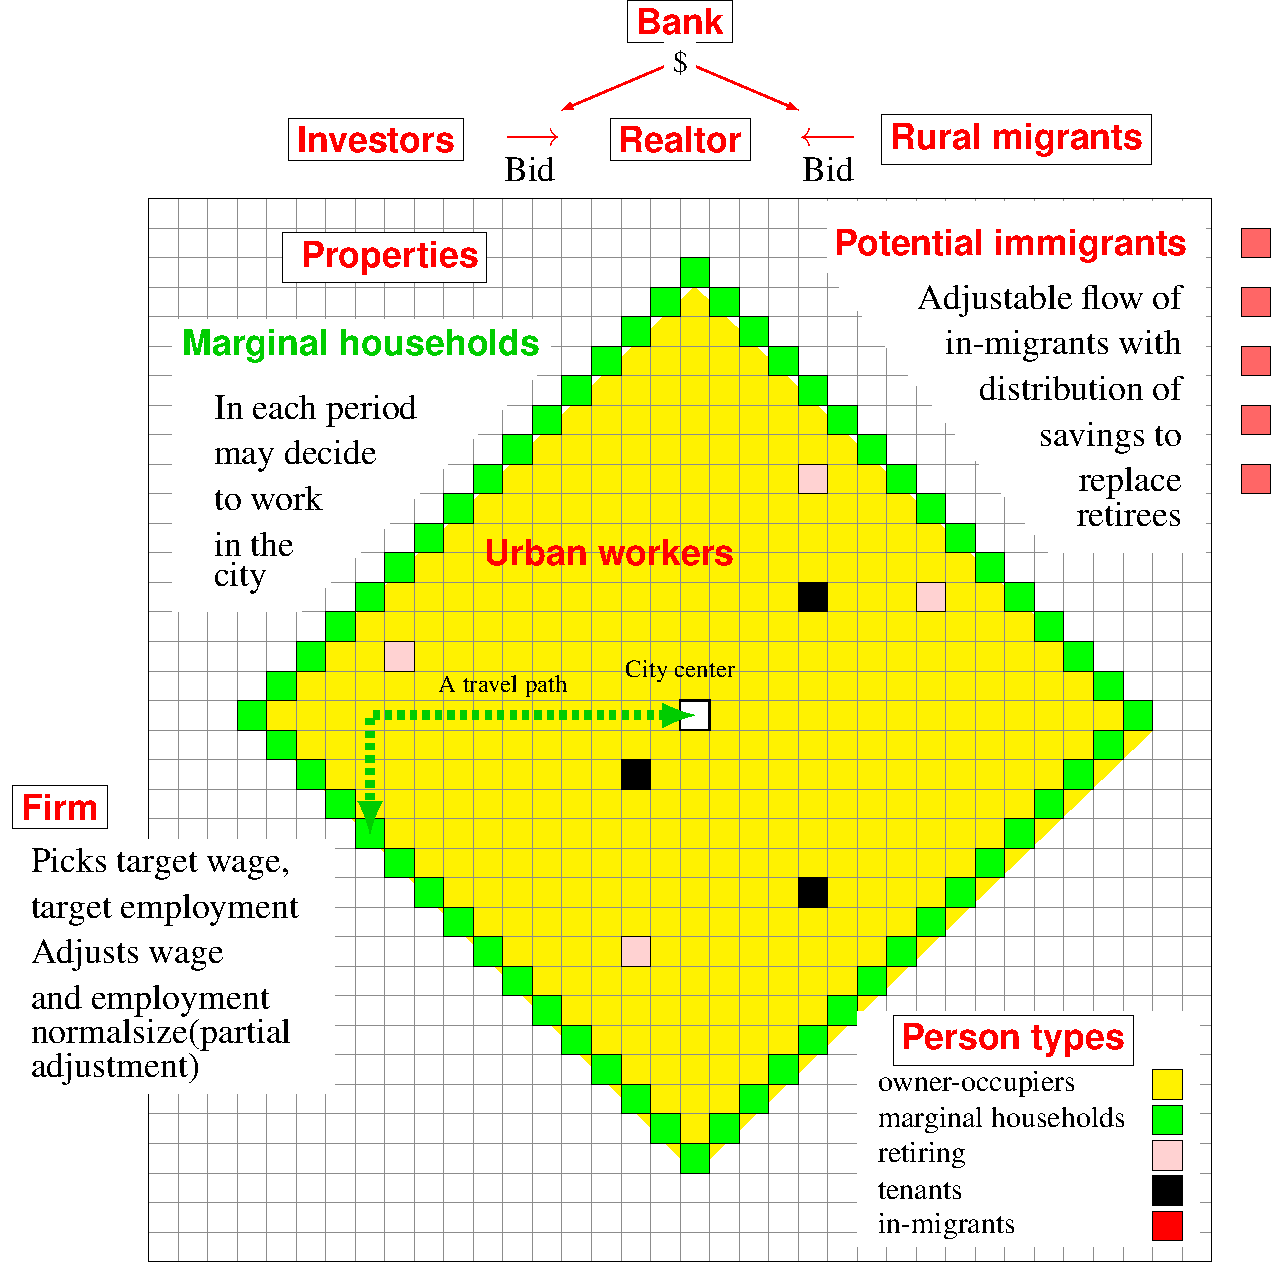
\includegraphics[width=1\linewidth]{fig/Kirsten_overview_figure.tex}
     \caption{Relationships among the agents in the model. The model operates on a grid of properties. Coloured squares make up the urban region. Owner-occupiers are yellow, tenants grey, and properites available for purchase because owners have retired are pink  Agents at the edge green decide in each period whether to participate in the urban labour market. In each period a pool of potential in-migrants may bid on the properties that are available. The firents without locations are shown outsid e of the }
\label{fig:Kirsten_overview_figure}
\end{figure}

% \centering
% \begin{figure}
%     \centering
%     \resizebox{16.5cm}{!}{%
%         
\tikzset{AgentStyle/.style={red, draw=black, font = {\Large\bfseries\sffamily}}}% Style for main lablels
\tikzset{TStyle/.style={red, font = {\Large\bfseries\sffamily}}}
\tikzset{ImmigrantStyle/.style={ purple!50!blue!70,  font = {\Large\bfseries\sffamily}}}
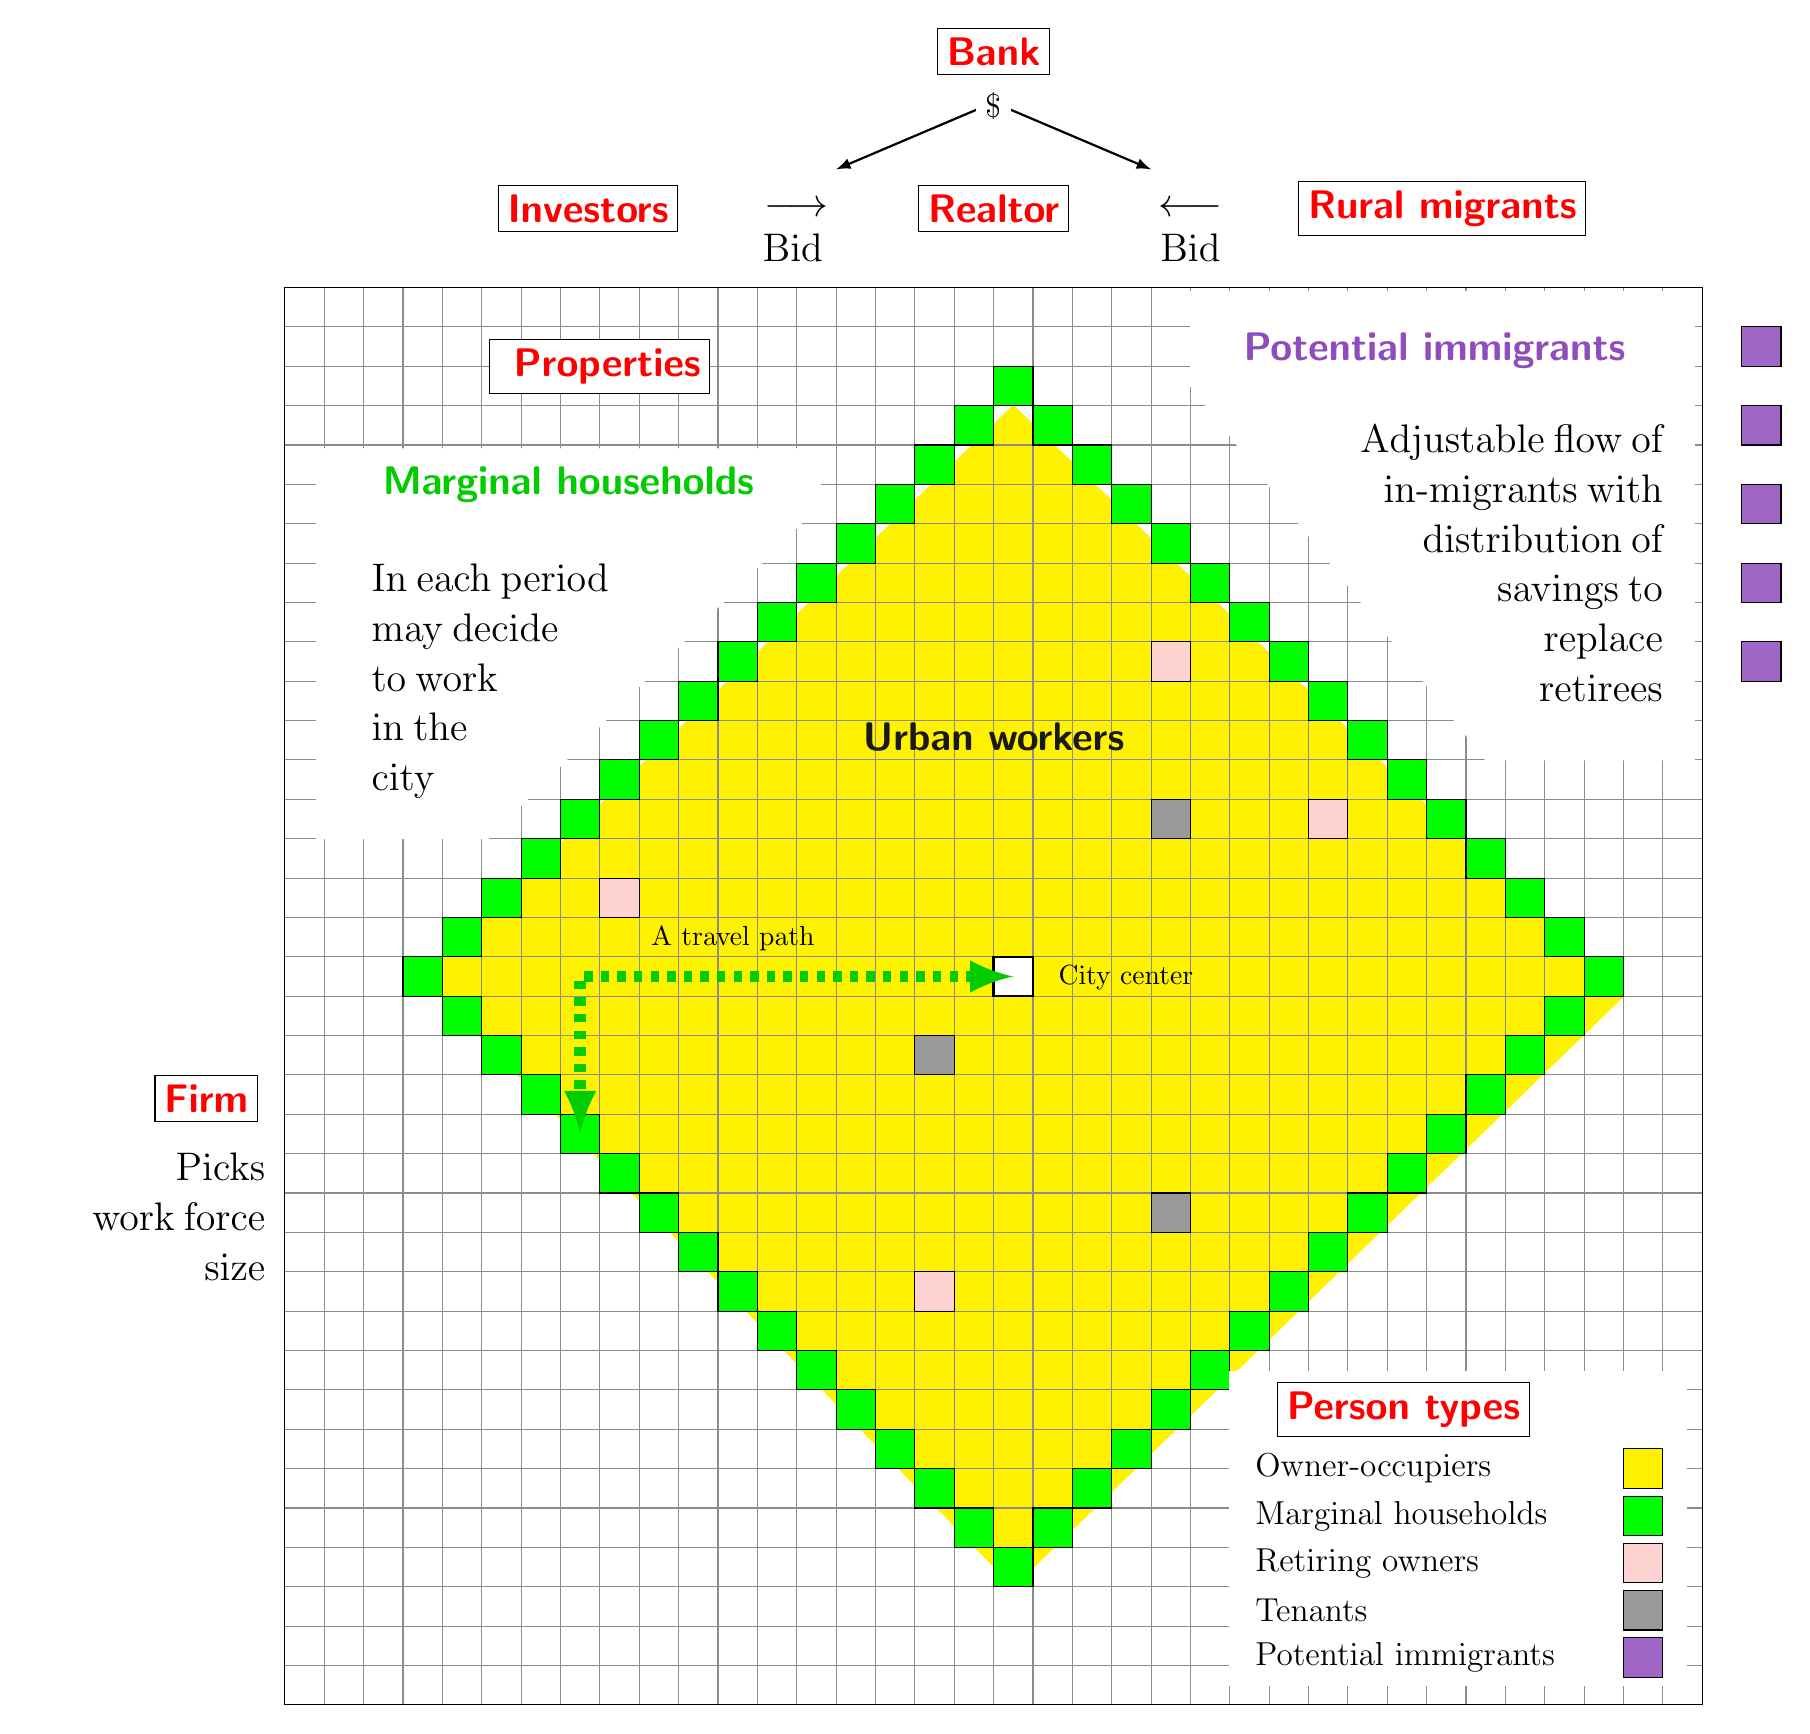
\begin{tikzpicture}
%\draw[very thin, gray!50, step=.5](-10,-10)grid(10,10);
% Locations for main label
  %Yellow square
 \draw [fill=yellow!80, yellow](8,0)--(.25,7.5)--(-7.25,.25)--(.25,-7.5)--cycle;  
 
 % grid 
  \draw[ thin, gray!90, step=.5](-9, -9)grid( 9, 9);
  \draw[  black, step=.5](-9, -9)rectangle( 9, 9);
  % center
 \draw  [fill=white, thick]  (0,0) rectangle +(.5,.5);
  \node at (1.68, .23) { City center};
  
% Marginal  residents _the green boundary
\foreach \z in {-7.5,-7,...,0}{ \draw  [fill=green] (\z,  {7.5+\z} ) rectangle +(.5,.5);} 
\foreach \z in {0,.5,...,7.5}{ \draw  [fill=green] (\z,  {-7.5+\z} ) rectangle +(.5,.5);}
\foreach \z in {-7.,-6.5,...,0}{ \draw  [fill=green] (\z,  {-\z-7.} ) rectangle +(.5, -.5);}  
\foreach \z in {.5,1,...,7}{ \draw  [fill=green] (\z,  {7.5-\z} ) rectangle +(.5,.5);}

% travel path
\draw [line width=1.5mm, latex-latex, dashed, black!20!green](.25, 0.25)--(-5.25,0.25)--(-5.25,-1.75);
\node at (-3.31,.73) {A travel path};


%.  Marginal households
\begin{scope}[shift={(-.4,0)}]
    \draw [fill=white, white] (-8.2, 6.95) --(-1.8,6.95)--(-1.8,6.25)-- (-6.02, 2)--(-8.2,2)--cycle;
    \node at (-5,6.5)[TStyle, black!20!green!100]{Marginal households}; 
    \node at (-5.5,4.)[text width=4cm] {\Large In each period \\may decide \\to work\\ in the\\ city\par};
\end{scope}
 
%  Firm
\begin{scope}
    \node [AgentStyle] at  (-10, -1.3){Firm};
    \node [text width=2.9cm, fill=white, align=right] at (-10.7, -2.8) {\Large Picks\\ work~force\\ size\par % \\normalsize(partial adjustment)
    };
 \end{scope}
 
 %Immigrants
     \begin{scope}[shift={(0,0)}]
     \draw [fill=white, white] ( 2.5,8.95) --(8.9, 8.95)--(8.9,3)-- (6.25, 3)--(2.5, 7.75)--cycle;
    \node at (5.6,8.2)[ImmigrantStyle]{Potential immigrants}; 
     \node [text width=6cm,  align=right] at (5.5,5.5) {\Large Adjustable flow  of \\ in-migrants with distribution of\\savings to\\ replace\\ retirees\par };
\end{scope}

% Locations for resident agents. (The first of these numbers is for the key.)
\def\retirees   {(2,4), (-5.,1), (-1,-4), (4,2)};			% retirees,   
\def\migrants {(9.5, 8), (9.5, 7),  (9.5,6.), (9.5,5.),   (9.5,4.)}; 	%potential migrants
\def\rental      { (2,2), (-1.,-1), (2.,-3)}; 			%rental properties

% Drawing resident agents.
\foreach \p in \retirees  {\draw [fill=pink!70] \p rectangle +(.5,.5);};
\foreach \p in \rental     {\draw [fill=black!40] \p rectangle +(.5,.5);};
\foreach \p in \migrants    {\draw [fill= purple!50!blue!60] \p rectangle +(.5,.5);};

% Labels and drawing for key for resident agents.
\begin{scope}[shift={(-.5,0.25)}]
    \draw [fill=white, white] ( 3.5,-5.02) rectangle (9.3,-9);
    \node at (4.1,-5.5) [right, AgentStyle]{ Person types};  %Title for key
    \node at 		(3.7,-6.25) [right]		{\large Owner-occupiers};
    	\draw [fill=yellow]    (8.5,-6.5) rectangle +(.5,.5);
	
    \node at 		(3.7,-6.85) [right]		{\large Marginal households};
    	\draw [fill=green]     (8.5,-7.1) rectangle +(.5,.5);	
	
    \node at 		(3.7,-7.45) [right]		{\large Retiring owners};
    	 \draw [fill=pink!70] (8.5,-7.7) rectangle +(.5,.5);
      
    \node at 		(3.7,-8.05) [right]		{\large Tenants};
    	\draw [fill=black!40  ]  (8.5,-8.3 ) rectangle +(.5,.5);	
	
    \node at 		(3.7,-8.65) [right]		{\large Potential immigrants };
    	\draw [fill= purple!50!blue!60]  	    (8.5,-8.9 ) rectangle +(.5,.5);	
\end{scope}

  \node [AgentStyle] at (5.7,10){ Rural migrants};
   \node [TStyle, black ] at (2.5,10){$\longleftarrow$};
  \node  [TStyle, black!90]  at  (0,3.3){Urban workers};
    \node  [AgentStyle, fill=white]  at  (-5, 8){\ Properties\ };

\node at (2.5, 9.5) {\Large Bid};
\coordinate (Realtor) at (0,10);

\coordinate (Workers) at (-2,2); %Angle left 

  \node  [AgentStyle] at (0,12) {Bank};  
  \node [AgentStyle] at (Realtor) {Realtor};
  \node  [AgentStyle]  at (-5.15,10){Investors };
    \node  [TStyle, black]  at (-2.5,10){ $\longrightarrow$};
  \node at (-2.55, 9.5) {\Large Bid};
%  \node  [AgentStyle]  at (Workers){Investors};

  \draw [black, thick, latex-latex](-2,10.5)--(0,11.35)--(2, 10.5);
  \node [fill=white] at (0, 11.3) {\large \$};

\end{tikzpicture}

%     }
% \caption{Relationships among the agents in the model}
% \label{fig:Kirsten_overview_figure}
% \end{figure}

\subsection{State variables}
State variables refer to the attributes of each kind of entity that vary over time. %\footnote{In the ODD framework, state variables commonly refers to both stock variables and parameters. Although it is inconsistent with usage in the analysis of dynamical systems, we follow the ODD convention in this section.}.
The entities in our model are the six agents types illustrated in Figure~\ref{fig:Kirsten_overview_figure}: 
\begin{enumerate}
    \item Persons, residents who are either owners or tenants on properties
    \item An investor who purchases housing for profit
    \item  A bank that provides financing for property buyers
    \item A realtor that manages property sales and finds tenants 
    \item An urban firm that provides employment and wages, and 
    \item Land units (properties or lots), which are locations to which persons are attached. 
\end{enumerate}

In Figure~\ref{fig:Kirsten_overview_figure}, agents are identified by black boxes around the agent type. Persons are classified by location, (as urban workers or rural workers), by ownership status (as owner-occupiers or tenants), or as in-migrants who may bid on properties that come up for sale. %The city grows when non-worker residents at the edge of the city are induced by a rising wage to begin commuting to the city center to work.
Persons are always associated with specific units of land. Each cell in the figure's grid is a land agent.  The number of person agents is equal to the number of land units plus a small pool of in-migrants temporarily located in the center of the city.

The investor, bank, realtor and firm are are \glspl{representative agent}. The are assumed to represent the actions of the entire class of agents of their type. 
 
Combined with rules for every agent these elements provide a simulation of an evolving city in a rural region. 

\subsubsection{Parcels of land are individual agents}

Because we have a spatial model, it is convenient to begin by describing the grid of properties representing a central city and a surrounding rural region. Each cell is a computational agent in the class of Land agents. Each cell has an address in a Cartesian space. Each has a set of attributes. Attributes that are adjusted as the model evolves are the state variables in the terminology of the documentation format we are using. Each cell is associated with one resident person-agent. %Properties are updated as the model evolves. 

The city is the subset of cells or the region over which workers choose to work at the urban center. The urban center is located in cell (0, 0). Properties are in the city, if the resident chooses to commute to work at the center of the city.  The city as a whole is not an agent. 

Each unit of land has an owner, either resident or non-resident, and a resident worker who may be an owner or a tenant. For simplicity, rural residents are always owners.  

When owner-occupiers retire or when investors choose to sell a property, it is listed for sale. The potential buyers are the investor and a selection of rural migrants with savings drawn from a distribution.  Low savings may limit the bid that the new resident can make. 

If no newcomer or investor purchases a listed property, the property remains on the market and a tenant is found. 

Attributes associated with each location are:
\begin{enumerate}[topsep=8pt,itemsep=3pt,partopsep=4pt, parsep=4pt]% ADDED NEW PACKAGE \usepackage{enumitem} AND REDUCED itemsep
    \item location,
    \item ownership type, 
    \item owner, with age and savings
    \item mortgage
    \item warranted price, 
    \item warranted rent, 
    \item appraised price, 
    \item realized price,
    \item price  change, 
    \item transport cost, 
    \item maintenance costs,
    \item tax rate,  
    \item density, 
\end{enumerate}
The last three,  maintenance costs, tax rate and density are the same for all properties in the current implementation. Transport cost combines location with a uniform cost per unit of distance.  The price variables are re-computed for properties when they are on the market when an owner retires or an investor decides to sell. Price change is used in expectation formation. % The owner may change


\subsubsection{Persons}
Rural and urban owner-occupiers and urban tenants belong to the agent class Person. Urban owner-occupiers have a 40-period working life, after which they retire and list their home for sale.  In the current implementation,  they are removed from the model. Perhaps they retire to the countryside. They could be allowed to age in place, but without relevant amenities there is a financial motive for moving out. % They could also be allowed to become landlords. %, but in the current implementation they would then be indistinguishable from other investors.

Marginal households are persons with properties at the edge of the city.  If the wage justifies travel to the city center, rural owner-occupiers may join the urban workforce as owner-occupiers. The geometry suggests there will be a discrete jump in population each time the wage passes a threshold, but the firms, target population is only allowed to adjust partially, which smooths population growth.

Newcomers are persons seeking to purchase or rent land and to join the urban workforce in each period. In the current implementation there are always enough newcomers to replace retirees. Each has savings, with the amount drawn from a distribution that allows at least some of them to bid on properties. If newcomers make a successful bid they become owner-occupiers. % If not, a newcomer may become a tenant. 
If they cannot purchase they are removed from the model. A new pool of newcomers is drawn in each period.  
Because computations are ordered by location, newcomers are arbitrarily associated with the center of the city at cell (0, 0).  

If an investor purchases a property, the rent it to a newcomer who then pays rent. If renters retire, they are replaced with new renters. If the investor chooses to sell, and an owner-occupier purchases the property, they displace the renter and move in.

For simplicity, individuals have the same preferences, employment opportunities and transportation costs.  Each person occupies one property.

The state variable of persons are location, ownership status, working period, and savings.  % Mortgage payments or rental payments are calculated to update savings. 
Other attributes include capital gains tax rate and borrowing rates. 

\subsubsection{Bank}
The bank is the sole member of the class of Bank agents. It sets maximum mortgage share and credit-worthiness using person attributes and bank parameters. It sets lending rates for persons and investors based on the prime rate. Mortgages payments are calculated for a 5-period term. The bank has no state variables.
 
\subsubsection{Investors}
% Investors are treated as a \gls{social class} with simple agency. 
There is one member of the class of Investor agents. 
The investor bids on all properties for which the calculated rate of return at least matches alternative investments. The investor draws on the global pool of capital. If the investor outbids tenants and newcomers, the property purchased is then owned by non-resident capital.  

The investor's decision-making is treated in detail in Chapter~\ref{chapter model}. Variables for the investor are the borrowing interest rate, properties owned, a capital gains tax rate, expectations about the rate of price change, and the maximum fraction of owned properties that may be listed for sale in each period. A fraction of investor-owned properties are listed for sale in each period. There are no  state variables, but the list of properties owned evolves. Investor wealth, the wealth of the class of investors, is calculated using the attributes of the properties, including price information.


\subsubsection{Realtor}
There is one member of the class of Realtor agents. 
The realtor keeps lists of properties for sale and for rent in each period, conducts bidding, and allocates properties to the winning bidder. The realtor interacts in each period with listed properties and all bidders. It's state variable is the data structure with the details of the property listings for properties currently for sale.

\subsubsection{Firm}
A representative firm is the sole member of the class Firm. The state variables for the firm are capital stock and workforce. At any price, wage, and cost of capital; the firm identifies target employment and capital stock. The targets are calculated using the rules derived from standard neoclassical firm theory. The firm then adjusts its current workforce and capital stock toward the target. 

The firm  is a price-taker: it does not set wages or output prices. Although the model employs a single representative firm to determine labour demand, we imagine that the wage adjustment process occurs in a decentralized and competitive market with many firms, each forced to adjust their own wage offer given excess demand or supply. This uncoordinated market response is captured in our model by a partial adjustment mechanism. 

%The production function is specified over  $N$, $A$, $alpha$, $beta$, and $gamma$. 
The target employment for the firm, multiplied by the number of firms gives the aggregate target labour. We term this value labour demand.  Demand is therefore planned employment rather than actual employment.  It is the number of posted job openings rather than the number of hires that firm actually achieve.  %Since the price of output is fixed, we can ignore output. %With perfectly elastic demand as assumed, the firm can sell any amount at the fixed price. 
Similarly, labour supply is the number of person agents who decide to work. The number changes as agents  near the edge of the city (marginal agents) decide to begin or stop work in the city or based on the previous period's wage. 
If labour demand exceeds the current population the wage is adjusted upward. Firms adjust to the revised wage in the following period.

The aggregation population $N$ used in the firm's production function differs from the aggregate firm workforce. In the current implementation, we compute the workforce as the number of cells that are urban, multiplied by the density. To account for the fact that not everyone who contributes to the agglomeration effect may work for firms, we add a seed population and scale the combination by a factor greater than one. The adjustment factors provide flexibility for later versions of the model.
     
\subsection{Scales}
This section describes the temporal and spatial resolution and extent of the model. 
We typically examine results for 100 cycles. Cycles are intended to roughly represent 100 chronological years of city.  Over that period our model city grows to approximately 2.5 million. The city does have an asymptotic limit, but since we are interested in financialization during periods of growth, parameters that control the scale have been chosen to let us examine the growth of a mid-sized city.  

The computational field is a grid of properties. To limit computational time, population is modelled coarsely and the size of the grid is restricted.  Grid size is typically a square 100-200 properties which, which is sufficient to contain the city while still leaving properties in the `rural' state in every direction after a typical 100 period run. 

Each cell has a single owner but represents a specific number of individuals for the population count and for the labour market. A density parameter is set at 100 so that the limited number of cells in the city provides a plausible urban population.\footnote{The density parameter is the simplest possible version of a density function, which is itself a simplification of a mixed population. At the cost of additional computation, properties can have individualized densities or can be subdivided to allow for more complex populations.}

The population determines the magnitude of the agglomeration effect that enters the firm's production function. Population is a function of density, the cost of transportation and the wage premium, which is determined by firm productivity. Transportation cost is the grid distance from the center. The distance is the sum of the absolute values of the x and y displacements from (0, 0), multiplied by the annual transport cost, which is set at 500 per cell-length. The transport cost per unit distance must be high enough to ensure that the city that emerges will remain within the boundaries of the grid in the course of a simulation run.

The firm's production function is subject to two conditions. First, the parameters $\alpha$  and $\beta$ must sum to less than one. Second, $\alpha +\beta + \gamma$ must be slightly larger than one.  The $\beta$ exponent is the labour-force-share of  firm revenue cost when we use a Cobb-Douglas production function. It is a scale factor in the or the wage and therefore controls the wage premium. We use a value in the range  0.7-0.8 that is consistent with typical values for developed countries. %{\color{red} ADD REFS} There is evidence that the share in national income has much lower over the last century.  
Different values do not change  our qualitative results, however.  


The representative firm is quite small, rising to about 60 workers. The number of firms is correspondingly large. 
Person agents have a working life of 40 cycles (years). Mortgage contracts are  for five years and are renewable.

The effect of modifying parameters of the financial system are discussed at length in Chapter~\ref{chapter-results}. 
The parameter space is large and the parameters interact to determine model variable such as population. We report variation around a single point in the parameter space to have easily compared results, however the results are consistent across a substantial region of the parameter space. % There is, a fairly large region of the parameter space that produces qualitatively equivalent results to those we report. 

\section{Process overview and scheduling}

\begin{figure}[h!tb]
\centering \vspace{-2cm}
 \begin{tikzpicture}[node distance=1.5cm]
\node (init) [startstop] {Initialization};
\node (interventions) [process, below of=init] {Model applies interventions};
% \node (record) [process, below of=interventions] {Record ownership share and reset counters};
\node (mainloop) [startstop, below of=interventions] {Main loop};
\node (firmupdate) [process, below of=mainloop] {Firm(s) update target employment, partially adjust workforce};
\node (wage) [process, below of=firmupdate] {wage adjusts for changed labour demand};
\node (land) [process, below of=wage] {Land records data and computes price forecast};
\node (actions) [process, below of=land] {People choose to work based on wages, retire, and list properties};
\node (investors) [process, below of=actions] {Investor lists properties};
\node (newcomers) [process, below of=investors] {Newcomers  bid on properties};
\node (bid) [process, below of=newcomers] {Investor bids on properties};
\node (realtors_sell) [process, below of=bid] {Realtor sells homes};
\node (realtors_rent) [process, below of=realtors_sell] {Realtor rents properties};
% \node (store) [process, below of=realtors_rent] {Model stores data};
\node (advance) [process, below of=realtors_rent] {Model stores data and advances time step};

\draw [arrow] (init) -- (interventions);
% \draw [arrow] (interventions) -- (record);
% \draw [arrow] (record) -- (mainloop);
\draw [arrow] (interventions) -- (mainloop);
\draw [arrow] (mainloop) -- (firmupdate);
\draw [arrow] (firmupdate) -- (wage);
\draw [arrow] (wage) -- (land);
\draw [arrow] (land) --(actions);
\draw [arrow] (actions) -- (investors);
\draw [arrow] (investors) -- (newcomers);
\draw [arrow] (newcomers) -- (bid);
\draw [arrow] (bid) -- (realtors_sell);
\draw [arrow] (realtors_sell) -- (realtors_rent);
\draw [arrow] (realtors_rent) -- (advance);
% \draw [arrow] (store) -- (advance);

\draw [arrow] (advance.south) -- ++(0,-.5) -- ++(7,0) |- (mainloop);
% % Custom arrow path
% \draw [arrow] ($(advance.south) + (0,-0.5)$) -- ++(0,-1) -- ($(mainloop.south) + (-2,-1)$) -- ($(mainloop.south) + (-2,0)$) -- (mainloop);

\end{tikzpicture}
\caption[Flow diagram for the agent based model]{Flow diagram for the agent based model.} \label{fig:computational-sequence}
\end{figure}


The model proceeds in discrete steps. Each time step represents one year. Agents of a particular kind execute their step function in randomized order and use state variables from the prior time step. Figure~\ref{fig:computational-sequence} illustrates the sequence. Figure~\ref{fig:information-flows} illustrates the major information flows between agents and functions.

% Persons initially have locations. They choose whether to work or not work, based on the wage premium and transportation costs, thus determining if their location is in the commuter-shed. This step determines the extent of the city and its population. Persons remain in the workforce until they reach retirement age. If people are above the retirement age, they retire and list any properties for sale if they are moving out of the city. 

% Agents are assumed to travel to the center to work only if the transportation of travel to the center is less than the extra pay earned for working at the center compared to the pay earned in rural occupation (the urban wage premium). 

% The sequence of the code means agents do not use information from, or interact with agents of the same type during their step function, so the order doesn't matter.
In each time step:

\begin{enumerate}
\item The representative firm computes the value of the marginal worker's value product at current prices, chooses a new target workforce.  It follows a partial adjustment rule in choosing current, labour force, capital stock for the following period. Firm size is constrained by diminishing returns to scale. New firms enter when population grow beyond what existing firms target. 

\item Aggregate current labour demand is computed, compared to existing supply, and a new wage is selected. 

\item The wage premium is calculated from the wage and used by agents to decide whether to work in the city.

\item Each lot, or unit of land, is an agent. Each uses the wage premium and its own location to compute its locational value, or warranted price, and potential rental earnings. 

\item The bank determines mortgage availability for newcomers and tenants. 

\item Newcomers and investors bid on properties listed for the period. They use an expected price that includes information about how the market has behaved, so it is possible for price bubbles and expectations to feed back into the dynamics. 

\item The realtor takes the list of bids and coordinates a bargaining process to reach a final price, if possible. 

\item If the new property owners do not choose to occupy their own houses, they rent the properties to newcomers as tenants. % who are included in the tenant count.
\end{enumerate}

% The illustration of the computational sequence in 
Figure~\ref{fig:computational-sequence} illustrates the computational sequence. % may make it difficult to understand the relationships among the agents in the model. In 
Figure~\ref{fig:information-flows} traces the economic relations among agents in the flow diagram.

\section{Design concepts} %LENGTH TRIPPLED
The model is intended to combine a theoretically grounded simulation of the spatial and temporal growth of a city with a new model of a housing market in which individual agents buy and sell property, live, work, and retire subject to a realistic financial system. 
To achieve this, not all the parts are modelled at the same level of resolution. We combine coarse generalizations about long-term agglomeration effects with fine-grained housing and financial market processes. 

\begin{figure}[h!tb]
\centering \vspace{2.5cm}
    \centering\vspace{-3cm}
% \tikzstyle{startstop} = [rectangle, rounded corners, minimum width=3cm, minimum height=1cm,text centered, draw=black, fill=red!30]
\tikzstyle{process} = [rectangle, minimum width=3cm, minimum height=1cm, text centered, draw=black, fill=orange!30]
% \tikzstyle{decision} = [rectangle, minimum width=3cm, minimum height=1cm, text centered, draw=black, fill=green!30]
% \tikzstyle{arrow} = [thick,->,>=stealth]


\begin{tikzpicture}[scale=.2,node distance=1.5cm]
\node (init) [startstop] {Initialization};
\node (interventions) [process, below of=init] {Model applies interventions};
% \node (record) [process, below of=interventions] {Record ownership share and reset counters};
\node (mainloop) [startstop, below of=interventions] {Main loop};
\node (firmupdate) [process, below=.5cm of mainloop, text width=5cm] {Firms update wages, number of workers, capital  based on prior wage};

    \draw [arrow] (init) -- (interventions);
    \draw [arrow] (interventions) -- (mainloop);
    \draw [arrow] (mainloop) -- (firmupdate);


\node (owners-retire) [decision, below=1cm of firmupdate, text width=5cm] {Owners retire};
\node (rural-boundary) [decision, left= 1cm of  owners-retire,  text width=4cm] {Boundary-adjacent owners  join or leave workforce};
\node (rural-remote) [decision,  right =1cm of owners-retire, text width=4cm] {Remote rural agents decide to join or leave workforce};


    \draw [arrow] (firmupdate) -- (rural-boundary);
    \draw [arrow] (firmupdate) -- (rural-remote);

\node (retired-list) [decision, below =.8cm of owners-retire, text width=5cm] {Retirees list properties};
  \draw [arrow] (owners-retire) -- (retired-list);



\node (Remote-bid) [process, right=1cm of retired-list, text width=4cm] {Remote rural agents bid for housing};
 \node (Invest-bid) [process, below=3cm of Remote-bid, text width=4cm] {Investors bid for housing};
    
%\node (invest-list) [process, green, below=6cm of rural-remote, text width=5cm] {investors list properties};land

\node (realtors_sell) [process, below = 1.5cm of retired-list ] {Realtors sell homes};
          \draw [arrow]  (retired-list) -- (realtors_sell);    
          \draw [arrow]  (Remote-bid) -- (realtors_sell.north east);     
\node (invest-list) [process, below=1.3cm of Remote-bid, text width=4cm] {Investors list properties};land
          \draw [arrow]  (invest-list) -- (realtors_sell);      
          \draw [arrow]  (Invest-bid) -- (realtors_sell.south east);               
            
\node (bank) [decision, below = 1.5cm  of realtors_sell, text width=5cm] {Bank  finances purchases};
        \draw [arrow] (bank) -- (realtors_sell);

\node (realtors_rent) [process, left = 1cm of bank, text width=4cm] {Realtors rent investor and empty homes};
        \draw [arrow]  (realtors_sell.south west) -- (realtors_rent.north east)   ; 
        
\node (tenant-adjust) [process, above=.5cm of realtors_rent, text width=4cm] {New tenants added to tenant list};

        \draw [arrow]  (realtors_rent) -- (tenant-adjust)   ;

\node (owner-adjust) [process, below = .7cm of rural-boundary,  text width=4cm] {New owners added to owner list};
  \draw [arrow] (rural-boundary) -- (owner-adjust);
  
\node (agglom-adjust) [process, thick, below = .5cm of owner-adjust, text width=4cm] {Agglomeration population adjusted};


  \draw [arrow] (realtors_sell.north west) -- (owner-adjust.south east);
\draw [arrow] (rural-remote) -- (Remote-bid);
 \draw [arrow] (owner-adjust) -- (agglom-adjust);
\draw [arrow] (tenant-adjust) -- (agglom-adjust);

\draw [arrow, line width=.5mm] (agglom-adjust.west) -- ++(-1.5,.5)  |- (firmupdate)node[midway,above right] {\Large Adjust population N}; 

\draw [arrow, red, line width=.5mm] (agglom-adjust.west) -- ++(-2.5,-.75)  |- (mainloop)node[midway,above right] {\Large Adjust productivity A}; 
%-- ++(0,-.5) -- ++(7,0) |-
%-- ++(0,-.5) -- ++(7,0) |-
% % % Custom arrow path
% % \draw [arrow] ($(advance.south) + (0,-0.5)$) -- ++(0,-1) -- ($(mainloop.south) + (-2,-1)$) -- ($(mainloop.south) + (-2,0)$) -- (mainloop);

\end{tikzpicture}


\caption[Main Agent decisions and information flows]{Agent decisions and information flows. Two feedback loops are emphasized. Firm decisions lead to adjustment of  population $N$,  which influences the agglomeration effects on firm productivity, and ownership changes affect the productivity prefactor $A$.}
\label{fig:information-flows}
\end{figure}

% Basic principles
% Adaptation - adaptive traits - rules for how changing in response to changes in environment or themselves. do they seek to increase some measure
% Objectives - what is the objective and how is it measured
% No - Learning - change adaptive traits based on experience
% Prediction - the anticipate based on past prices

The principles explored include the relationship between urban agglomeration effects and the financialization of the urban housing market. To explore these principles, we combine two distinct approaches to modelling social systems: agent-based and equilibrium-oriented economic modelling. 


\subsection{Convergence to equilibrium}
To bypass the complex and partially understood wage-setting process we convergence to equilibrium conditions for the firm internally and for labour markets. In this approach, we do not assume that the agents are constantly achieving equilibrium or even that decisions are correct, only that they represent adjustments in the correct direction. We assume that the firm is setting targets for its workforce and capital stock intended to achieve maximum profit, then adjusting partway toward those targets. Similarly, while demand for labour is determined by the collection of firms, supply is determined by the response of potential workers to the level of the wage. We allow the wage to move upward if there is excess demand or downward if there is excess supply.

This partial adjustment process evades the common criticism of equilibrium modelling that it requires perfect information and perfect rationality.  

In the housing market, investors also seek to maximize their profits. They calculate the return on their investments accurately (up to the limits of their knowledge) over a 5-year mortgage period. Our treatment of how they form expectations about the potential capital gains is frankly simplistic. We assume that the expected price change over a 5-year mortgage period is just a linear projection of the rate of change in the previous period.  

We also use equilibrium arguments to compute land rents from the transportation cost and urban wage premium that drive urban locational decisions. Realistically, like capital gains, the rents that can be extracted are a slow-moving target that is difficult to forecast. We essentially assume that marginal agents and potential buyers accurately estimate their annual travel costs and local rents, and do not face fixed costs of change.   %This is a convenient fiction that matters far less than the omission of urban amenities (see Appendix~\ref{chapter-amenity}), variation in family type, or density.  

Chapter~\ref{chapter-methodology}, on methodology, provides more detail about the methodological decisions that inform the modelling decisions. 

% The model also expresses several the other concepts as described below. 

\subsection{Emergence}
% The class structure is emergent in our model, in that it's not in the base sent of specified objects, but it is a structure that appears through the interaction of agents in the model rather than one specified initially.

% PI "today's theoretical physics is tomorrow's technology"

% Roemer defines class as 
% class relations are determined by individuals' ownership or non-ownership of productive assets, such as labour,  machinery, factories, or, in our case, land. Exploitation occurs when someone gets their income from the productivity of someone else's person or assets. 

% In this sense, 
The city is an emergent entity that arises out of the rural economy as a result of agglomeration economies. The social structure is also emergent. We begin our exploration after the city and a two-class structure has emerged. We then examine how their class structure evolves. The classes are:
\begin{enumerate}
    \item Rural owner-occupiers.
    \item Urban owner-occupiers.
\end{enumerate}
Members of both classes own the land they live on. Urban owners differ in that they have access to an urban labour market. We do not specify whether rural owners gain an income as producers for example, as peasant owners, or as labourers. The logic of the migration equilibrium requires all agents be equally well off. The urban owners are a mixed class in the sense that they sell their labour like classic proletarians but also own a valuable capital asset, which is their land. Introducing additional differences among agents would open the possibility  the endogenous emergence of further \gls{class} distinctions based on access to various forms of capital, a process explored by John Roemer in his General Theory of Exploitation and Class \cite{roemerGeneralTheoryExploitation1982}.

Two more classes emerge in our simulations:
 \begin{enumerate}    \setcounter{enumi}{2}
    \item Urban tenants.
    \item Investors. 
\end{enumerate}
There are now two possible pure urban regimes, an owner-occupier regime and a tenant regime, in which investors own all properties. We start our experiments with a pure owner-occupier regime in which those who own houses and work can build equity.  The city may then transition toward the investor-owned regime as investor-agents purchase properties based on local expected financial return calculations. Our experiments explore some policy interventions that could affect the transition.


% Ownership, the regime, emerges, advantage are amplified leading to a different end state.They correspond to social classes  



%We model individual agents' access to finance, %and the cost of money we introduce an innovation to formal urban modelling. We 
%drawing on the literature for the relevant `\gls{stylized facts}' about differences in individual financial access based on wealth and income. 

\subsection{Sensing}
All agents have lagged information about the wage. They observe job postings by firms. They know their own savings and borrowing costs. They can calculate  warranted price and expected price growth.% They make their decisions based on what is best for themselves, based on their computations. 



\subsection{Adaptation, learning and prediction}
There is no learning in the sense that agents do not change their traits based on experience. Agents do, however, make predictions, anticipating prices based on the rate at which those prices have increased in the past, with the prediction variable $\dot P$.

\subsection{Interaction}
Agents make decisions to work, retire,  purchase, or invest independently but because of agglomeration effects, their decision to work and its effect on the size of the labour market feed back to affect wages and the decisions of others in the next step. 

The central interaction is in the housing market through the competitive bidding process that allocates properties and rents.  A secondary, parametric interaction occurs if the allocation of housing or rents influences the production function as described in chapter~\ref{chapter-tramsmission}.

\subsection{Stochasticity}
Agents do not face uncertainty. Stochasticity comes into the main model two ways: through the distribution of agents' initial savings, and through randomizing the order in which agents act. 
% When multiple runs are made with the same parameter settings, these stochastic elements only produce variation in the evolution of the ownership ratio if the ownership ratio affects productivity. With linkages, all the outcome variables will vary slightly.

% For testing the model's sensitivity to parameters, we use a version that shortcuts the land market and bidding process by directly calculating equilibrium population.  This version lacks the stochastic elements built into the land market sub-model. It is much faster computationally.

\subsection{Feedback loops}
Feedback loops are not part of the ODD standard, but are an important concept in this work.\footnote{Feedback loops are a fundamental feature of almost all systems. They have probably been recognized by theorists for centuries. Marx, to take one relatively modern example, identified the growth dynamic of the capitalist system as a feedback loop, with capital investments producing a surplus that was fed back into investment, growing the stock of capital. Marx claimed that this loop produced dynamic instability and a great deal of subsequent work has supported his insight \cite{dumenilStabilityInstabilityDynamic1986} \cite{schumpeterInstabilityCapitalism1928}. More recently, the Keynesian multiplier is a result of feedback in macro models between expenditure and jobs. That loop produces a stable equilibrium. Neoclassical growth theory built on that mechanism to explore the determinants of economic growth using differential and difference equations. \cite{radzickiIntroductionFeedbackEconomics}} 
% https://en.wikipedia.org/wiki/James_J._Kay
% https://www.researchgate.net/scientific-contributions/James-J-Kay-2162967174
% https://uwaterloo.ca/systems-design-engineering/about-systems-design-engineering/department-history
There are three \glspl{feedback loop} in the model: 
\begin{enumerate}
    \item the productivity-wage, population-productivity loop that we call the Alonso-Jacobs cycle,
    \item a speculative price-expectations cycle that may produce price bubbles, 
    %\item a price-financialization feedback that directly changes the ownership pattern in the urban housing market.
    \item the hypothesized feedback from financialized ownership to the production function, which depresses wages, reduces growth and therfore inhibits financialization.
 
\end{enumerate}
 % Forrester, the creator of system dynamics computer simulation modeling, argued that change over time is caused by the process of accumulation CITE.
% The feedback concept formally entered the social sciences through two channels: cybernetics, pioneered by Nobert Wiener  and the participants of the Macy Foundation Conferences, and the servomechanism/control engineering thread championed by Jay W. Forrester and others. Both threads were picked up and applied by prominent economists.\footnote{Richardson \cite{richardsonFeedbackThoughtSocial1991} mentions Oscar Lange (1970), Kenneth Boulding, and Alfred Eichner, Phillips,  R. G. D. Allen (1956), and Axel Leijonhufvud.} There is now a niche sub-discipline in economics called ``Feedback Economics'' \cite{radzickiIntroductionFeedbackEconomics, cavanaFeedbackEconomicsEconomic2021}. %  and a great deal of work in The servomechanism/control engineering thread is the one most closely related to \gls{system dynamics} modeling and to ideas used in this thesis.

 
% Our model incorporates two important feedback loops. One, driven by agglomeration, we call the \Gls{Alonzo-Jacobs cycle}. The other is 
The loops are linked. Rising productivity raises wages, which then works through two paths. It can raise rents, effectively transferring productivity gains to landowners, and it can draw more workers into the city workforce, enhancing the \Gls{Alonzo-Jacobs cycle}. 
\
%A rapid increase in housing prices may choke off urban population growth and cause the \Gls{Alonzo-Jacobs cycle} to stall. Rapid expansion of the housing stock should have the opposite effect. 
Much depends on the speed of response of the city population and the rate of transmission of agglomeration effects to wages through the firm. Our base model allows the boundary to respond to increments in the wage with a small lag. In the base model, financial flows are unrestricted but the rate of financialization is limited by the rate of turnover of ownership. We parameterize the rate of adjustment for each of the stocks in a simple way to faciltate sensitivity analysis.

\subsection{Observation}
% The model records a large number of computed variables for diagnostic purposes.
The output variables we report are the urban wage, land prices, city size, owner-occupier population, tenant population, total urban population, who owns which property, previous prices, firm capital stock, firm workforce size, and number of firms.

\section{Initialization}
Initial values for the model are detailed in Appendix~\ref{appendix-parameters} on initial values.

\section{Input}
Parameters have been chosen to be in ranges consistent with theory and, where possible, empirical work. The combination of parameter values for the production model was chosen to produce a plausible growth trajectory for a city that grows from small to large over a reasonable time period. To model interventions, we change key parameters mid-run to represent shocks to the system, such as labour market shocks, price shocks, and cyclical patterns. % We do discuss the settings or the calibration process because the production model is simply the environment for  our agent-based exploration of the housing market.  % time varrying data. 
The model does not draw on outside digital datasets. 

\section{Submodels}
We have described our model in terms of a few major components: the Alonzo-Jacobs model, the financial sector, and the housing market.  The large components themselves each rests on a large number of modelling decisions that we have discussed in Chapters~\ref{chapter-introduction}  through \ref{chapter-model}. We prefer to think of these as sub-models rather coding decisions because each is derived from theoretical or empirical considerations based on our readings of the literature (which is often extensive, varied, and inconclusive). They are also influenced by pragmatic decisions about how to keep the overall model simple and model. Individual submodels can be modified or replaced to reflect different assumptions or conditions.
 
\begin{enumerate}
    \item The spatial structure of the model, with each land unit having a transportation cost based on linear distance from the urban center;
    \item The population model, with a uniform density of owners or tenants located spatially; 
    \item The overlapping generations lifecycle model with retirement after 40 years;
    \item the population replacement model, 
    \item the population determination model driven by decentralized agent decisions;
    \item The representative firm model that generates the labour demand. This includes a specific production function and a model of how a profit-maximizing firm hires inputs and how rapidly it adjusts;
    \item The firm entry model that adjusts the number of firms toward the number of optimally sized firms the populations will support;
    \item The aggregate firm sector model that determines labour demand for the entire city as the representative firm demand times the varying number of firms;
    \item The perfectly elastic export demand for output model; 
    \item A household decision-making model that determines whether individuals work in the city based only on the wage and transportation cost for each property; 
    \item the agglomeration model that augments firm productivity based on a function of the number employed;
    \item The land valuation models used by agents; 
    \item The price expectations model;
    \item The land market model in which homeowners and financialized investors bid on properties for housing or to capture the rising rents due to agglomeration;
    \item The auction model that allocates properties and generates property prices for each period.
\end{enumerate}


% \section{DIAGRAMS AND FLOW}

% Initialization
% Apply interventions
% Record ownership share and reset counters

% Main loop
% Firms update wages based on how many people choose to work in the city
% Land records locational rents and calculates price forecast
% People decide whether to work, retire, and list properties to sell
% Investors list properties to sell
% Create newcomers to purchase properties for sale
% Investors bid on properties
% Realtors sell homes
% Realtors rent properties
% Store data
% Advance model


\section{Expectations}
\Glspl{expectation} introduce a mental model of the future state of agents into current decisions.  We employ a simple backwards-looking expectation formation anchored 
%  This ANCHORING IS INTERESTING, BY THE WAY
to current rental returns.\footnote{Forecasts based on recent price movements can give rise to \glspl{price bubble} through either speculative or precautionary motives. Expectations anchored in \gls{perfect foresight} have different dynamics since agents correctly forecast the path of prices \cite{muthRationalExpectationsTheory1961}.  We describe an investment rule of this sort in Chapter~\ref{chapter-financialization} on financialization.} 



%Combining a spatially explicit agent-based model of the housing market with equilibrium models of rent and urban production allows us to stay close to the analytic tradition, and connect the work with both classical and neo-classical theory. 
% As pointed out above, we rely on equilibrium arguments in our model to ``black box'' the production sector and most of the labour market, including most decisions by producers and wage demands by workers.  


% \subsubsection{SORT - single value frontier - explore reasons}
% WHERE TO EXPAND% *** We will explain why the rent charged to the tenant is locked  to a single value. A few factors - we are looking at the frontiers- the economically justified maximum as a way of linking productivity and extraction formally. - there are many variations and extensions to build on/explore/relax these core assumptions - - want to do this for a few reasons \dots



%  It follows that 
% \[\frac{\partial U_i(d, d(dots)}{\partial t}=\frac{\partial U_j(d, /dots)}{\partial t}\]
% Finally, our model of the financial sector falls between the two approaches: each property transaction decision is made individually as it would be in an agent-based model, but we don't track individual investors. Our investor is technically an agent in the agent-based modelling sense, but the agent is the entire class of financial investors in housing, which is to say, a representative agent. Interestingly, perhaps, each property is also formally an agent with a set of attributes such as location, density, and ownership status. 





% \subsection{Marginal vs inframarginal quantities}
% In relying on these equilibrium conditions, we are implicitly applying standard neoclassical economic methods although our focus is not on the \gls{marginal} conditions that determine prices, but on the \gls{inframarginal} quantities that make up rents. We can illustrate with a diagram that illustrates the disnction between marginal and inframarginal (explained in more detail in Chapters~\ref{chapter-rent} and \ref{chapter-space} on rent and space respectively). 

% \vspace{.3cm}
% \begin{figure}[h!t!]
% \centering
% 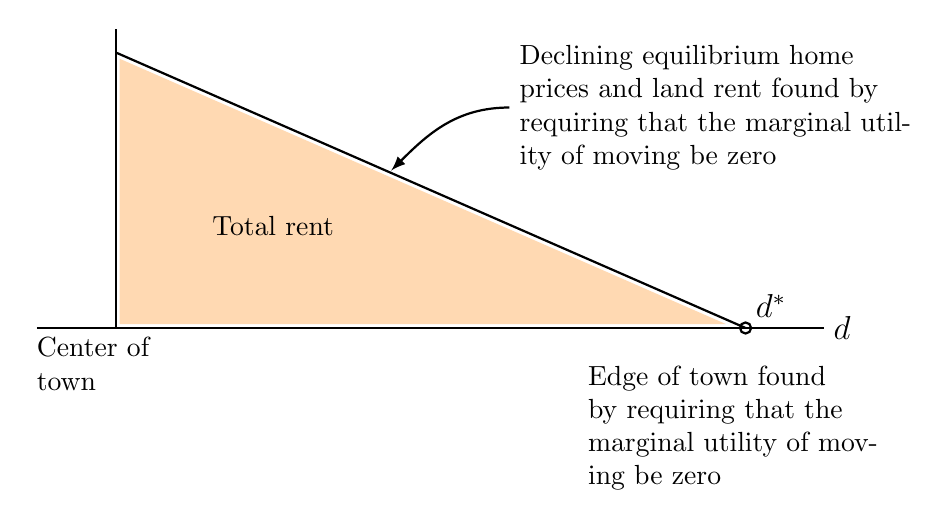
\begin{tikzpicture}[domain=0:2]
%\draw[thick,color=gray,step=.5cm, dashed] (-0.5,-.5) grid (3,3);
\draw[line width=.01] (0,0) -- (10,0) node[right] {\large $d$};
\node at (1,0) [below,text width=2cm] {Center of town};
%\draw[thick ] (0,3)node[above right] {merchant's price in town} -- (10,3) ;
\draw[thick ] (0,0)  -- (10,0); 
\draw[thick, -latex] (6,2.8)
node[right, text width=5cm]{Declining equilibrium  home prices and land rent found by requiring that the marginal utility of moving be zero} 
to [out=180, in=45](4.5,2); 

\fill[orange!30] (1.05,0.05)--(8.75,0.05)--(1.05,3.42)--cycle;

\draw[thick ] (1,0) -- (1,3.8);
\draw[thick ] (9,0)node [above right]{\large $d^*$}circle[radius=2pt] node[below=.35cm,text width=4cm] {Edge of town found by requiring that the marginal utility of moving be zero} -- (1,3.5) ;

\node at (3,1.3){Total rent};
\end{tikzpicture} 
% \caption{Illustrating marginal and infra-marginal quantities with the bid-rent curve and aggregate rent.}
% \label{fig-land-rent-as-inframarginal}
% \end{figure}

% In Figure~\ref{fig-land-rent-as-inframarginal}, The level of rent is determined at any distance by individuals making comparisons locally. At point $d,^*$ the person at the edge of the city decides whether to work in the centre or in the non-urban space. These are \gls{marginal} decisions. The orange area represents the total rents generated between $d=0$ and $d=d^*$. It is a summation of \gls{inframarginal} rents. Like Ricardo \cite{ricardoEssayInfluenceLow1815}, we are concerned with the distribution of rents, an inframarginal quantity.


% \subsection{Coarse graining}

% Using agent-based models, combined with simple equations is also one appraoch to coarse graining. 
% There's a distinction between coarse grained and fine grained models. Equation~\ref{eqn-population-output}  is a high-level generalization---a ``coarse-grained'' model. Modelling always faces a trade-off between computational tractability and representing details. \cite{GET_TerrysDissertation, GET_PaulsBook}

% Coarse-grained models must capture the stylized facts. %, as ours does.

% where the model is insenstitive to the details, you really want a representation that's small that captures the big pattern. 
% When you move to getting the details of the model, you know you have a model that tracks the observable. 
% Sometimes the model is sensitive to the details, and a more fine grained model is needed. There is an advantate to having a continuum of models that make it posible to represent systems with different levels of nuance/detail. We are focused on modelling a coarse grained model of the production system.
% % \section{SORT}
% % providing tractable models.  equilibrium analysis of marginal effects, and representative agents which hid distributional effects, as well as spaceless economic models of markets made it difficult to capture the richer spacial dynamics of urban rents, and the details of the ways economic forces play out for individual actors.

% % First they've not tended to build in, in a sophisticated way classical economic theory,
% % In general, classical economic theory has not been developed in agent-based modeling work
% % Agent-based models have begun with simple models, using and relaxing neoclassical assumptions, and building from first principles. This is absolutely the place to start. As the field matures, it makes sense to introduce theory in a more nuanced way, that connects with classical theory/the history of thought, etc

% % Second, relatively little agent-based modelling work integrates with the neoclassical economic work in a way that makes the relation clear/holds the advantages. ABM work tends to both reject neoclassical approaches and rely on neoclassical assumptions.
% % More generally only a few agent models (e.g. spruce budworm) connect the analytic and agent models in a clear rigorous way. We focus on holding in addition to the relation with classical theory, a close connection with the many advances made withing neoclassical modelling

% % - this connection will make it easier to incorporate in teaching and for mainstream economists to engage on and build with.

% % This work builds, first, a simple conceptually clear model tightly integrated with the core economic modelling traditions, that builds on the theory of rent.

% % ALSO (Agent modelling also tents to model individuals- we also take some steps to agent-based modelling beyond the individual, and to the work developing model in a mode ideas)

% % Third, econ lacks resilience analysis and models, yet hysteresis clearly present in the relation between the built environment and econ activity. Although there's been work on dynamics and individual effects, there has been little work looking at the resilience dynamics in economic models, we take that approach looking at the resilience of community and individual wealth, and the relationship between that wealth and productivity. 

% % - This puts resilience dynamics at the center of economic analysis.

% % The resilience analysis looks at the dynamics of rent in economic boom and bust cycles.
% % There is a ratchet effect, achieved through hysteresis in the system, in which sucks wealth out of communities on the way up and on the way down. % DETAIL ONCE DRAFTED.


% % The emphasis is on clarity and connecting with the equilibrium in economics, and systematically relaxing each, to connect with the analytic tradition of economic modelling
% % The clarity of intuition of the neoclassical tradition with the deeper root of distribution theory rooted in classical economics and the breath and rigor possible with new tools from the study of complexity and statistical physics.
